% Figuras de contexto del Bloque 1 — Afirmaciones 1 y 2
% Fuente para render-tikz-for-html.ps1 → genera FIGURA_1 ... FIGURA_6
% FIGURA_1 = Item 2 (S en (10,6) r=6)
% FIGURA_2 = Item 3 (zona bolsa de arena, centro (8,6) r=5)
% FIGURA_3 = Item 4 (antena T en (7,5) r=5)
% FIGURA_4 = Item 5 (antena H en (4,5) r=2 — figura inicial)
% FIGURA_5 = Item 6 (barco R en (5,3) r=1, puerto P en origen)
% FIGURA_6 = Item 7 (dispositivo V en (8,4) r=4, lab L en origen)

\begin{tikzpicture}[scale=0.34]
  \draw[<->, thick] (-2,0) -- (18,0);
  \draw[<->, thick] (0,-2) -- (0,15);
  \node[anchor=west] at (18.4,-0.8) {x (este)};
  \node[anchor=south east] at (3.5,15.5) {y (norte)};
  \draw[dashed] (10,0) -- (10,6);
  \draw[dashed] (0,6) -- (10,6);
  \draw[thick] (10,6) circle (6);
  \fill (10,6) circle (0.35) node[above left, inner sep=2pt] {S};
  \node[anchor=north] at (10,0) {$10$};
  \node[left] at (0,6) {$6$};
\end{tikzpicture}

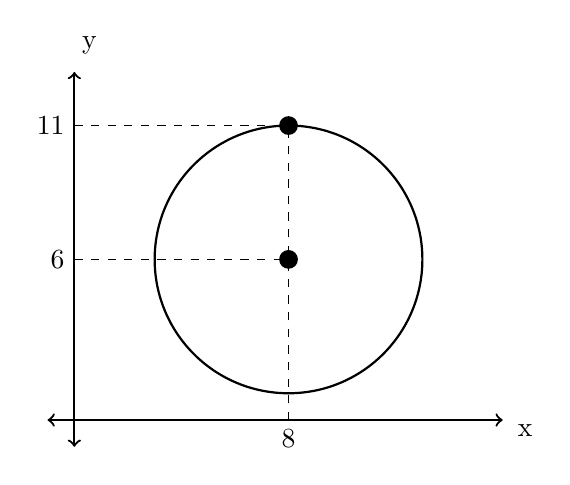
\begin{tikzpicture}[scale=0.34]
  \draw[<->, thick] (-1,0) -- (16,0);
  \draw[<->, thick] (0,-1) -- (0,13);
  \node[anchor=west] at (16.2,-0.4) {x};
  \node[anchor=south east] at (1.2,13.3) {y};
  \draw[thick] (8,6) circle (5);
  \draw[dashed] (8,0) -- (8,11);
  \draw[dashed] (0,6) -- (8,6);
  \draw[dashed] (0,11) -- (8,11);
  \fill (8,6) circle (0.35);
  \fill (8,11) circle (0.35);
  \node[anchor=north] at (8,0) {$8$};
  \node[left] at (0,6) {$6$};
  \node[left] at (0,11) {$11$};
\end{tikzpicture}

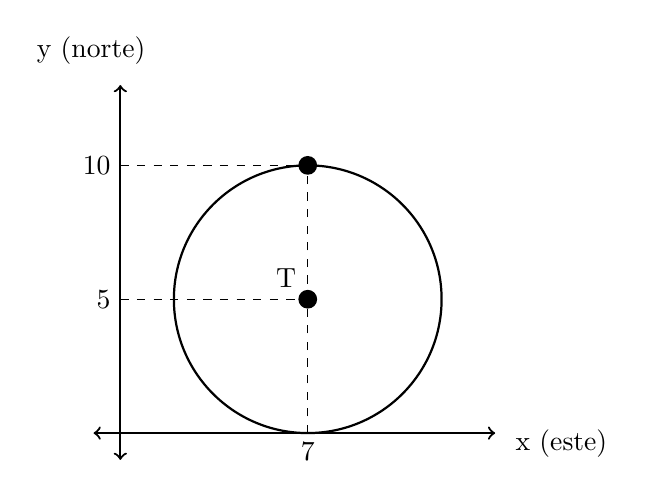
\begin{tikzpicture}[scale=0.34]
  \draw[<->, thick] (-1,0) -- (14,0);
  \draw[<->, thick] (0,-1) -- (0,13);
  \node[anchor=west] at (14.4,-0.4) {x (este)};
  \node[anchor=south east] at (1.3,13.4) {y (norte)};
  \draw[thick] (7,5) circle (5);
  \draw[dashed] (7,0) -- (7,10);
  \draw[dashed] (0,5) -- (7,5);
  \draw[dashed] (0,10) -- (7,10);
  \fill (7,5) circle (0.35)
    node[anchor=south east, inner sep=2pt, xshift=-2pt, yshift=2pt] {T};
  \fill (7,10) circle (0.35);
  \node[anchor=north] at (7,0) {$7$};
  \node[left] at (0,5) {$5$};
  \node[left] at (0,10) {$10$};
\end{tikzpicture}

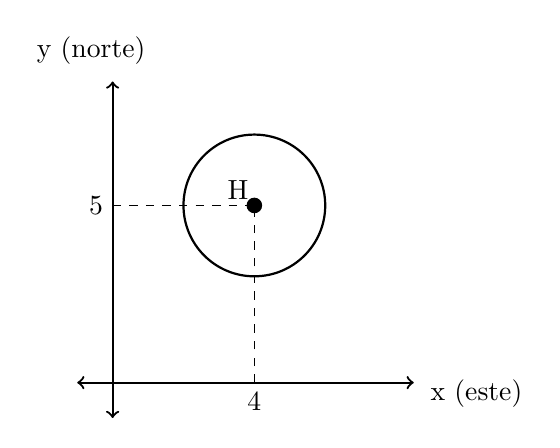
\begin{tikzpicture}[scale=0.45]
  \draw[<->, thick] (-1,0) -- (8.5,0);
  \draw[<->, thick] (0,-1) -- (0,8.5);
  \node[anchor=west] at (8.7,-0.3) {x (este)};
  \node[anchor=south east] at (1.2,8.7) {y (norte)};
  \draw[thick] (4,5) circle (2);
  \draw[dashed] (4,0) -- (4,5);
  \draw[dashed] (0,5) -- (4,5);
  \fill (4,5) circle (0.22)
    node[anchor=south east, inner sep=2pt] {H};
  \node[anchor=north] at (4,0) {$4$};
  \node[left] at (0,5) {$5$};
\end{tikzpicture}

\begin{tikzpicture}[scale=0.65]
  \draw[<->, thick] (-1,0) -- (7.5,0);
  \draw[<->, thick] (0,-0.5) -- (0,6.5);
  \node[anchor=west] at (7.7,-0.3) {x (este)};
  \node[anchor=south east] at (1.1,6.7) {y (norte)};
  \fill (0,0) circle (0.18) node[below left, inner sep=2pt] {P};
  \draw[thick] (5,3) circle (1);
  \draw[dashed] (5,0) -- (5,4);
  \draw[dashed] (0,3) -- (5,3);
  \draw[dashed] (0,4) -- (5,4);
  \fill (5,3) circle (0.18)
    node[anchor=south west, inner sep=2pt] {R};
  \fill (5,4) circle (0.18);
  \node[anchor=north] at (5,0) {$5$};
  \node[left] at (0,3) {$3$};
  \node[left] at (0,4) {$4$};
\end{tikzpicture}

\begin{tikzpicture}[scale=0.46]
  \draw[<->, thick] (-1,0) -- (14,0);
  \draw[<->, thick] (0,-0.5) -- (0,10.5);
  \node[anchor=west] at (14.2,-0.3) {x (este)};
  \node[anchor=south east] at (1.2,10.7) {y (norte)};
  \fill (0,0) circle (0.175) node[below left, inner sep=2pt] {L};
  \draw[thick] (8,4) circle (4);
  \draw[dashed] (8,0) -- (8,4);
  \draw[dashed] (0,4) -- (8,4);
  \draw[dashed] (8,4) -- (8,8);
  \draw[dashed] (0,8) -- (8,8);
  \fill (8,4) circle (0.175)
    node[anchor=north east, inner sep=2pt, xshift=2pt, yshift=-2pt] {V};
  \fill (8,8) circle (0.175) node[above right, inner sep=2pt] {C};
  \node[anchor=north] at (8,0) {$8$};
  \node[left] at (0,4) {$4$};
  \node[left] at (0,8) {$8$};
\end{tikzpicture}
